\section{Introduction}

\begin{frame}{Introduction: Problem Statement}
\begin{itemize}
    \setlength\itemsep{1.5em}
    \item There are $K$ seats with a booking window of $T$ days.
    \item Design a policy, $p_t, t \in \{1, 2, \ldots, T\}$ that will maximize the revenue over the booking window.
    \item Demand for seats at price $p_t$, denoted by $d(p_t)$, is a random variable supported on positive integers.
    \item Use RL to learn the optimal policy in case demand function is unknown.
\end{itemize}
\end{frame}

\begin{frame}{Introduction: Demand Function}
\begin{itemize}
    \item On any given day, we want to sample an order for a number of seats. The total order can be represented as a non-negative integer.
    \item The demand function should ideally depend on a positive real-valued price and a source of randomness.
    $$d: \mathbb{R}^+ \times U \rightarrow \mathbb{Z}^+ \cup \{0\}$$
    \item One way to capture the dependence on price is by changing the mean of the distribution of demand function as a function of the price.
\end{itemize}
\begin{figure}
    \centering
    \hfill
    \begin{subfigure}[t]{0.475\textwidth}
        \centering
        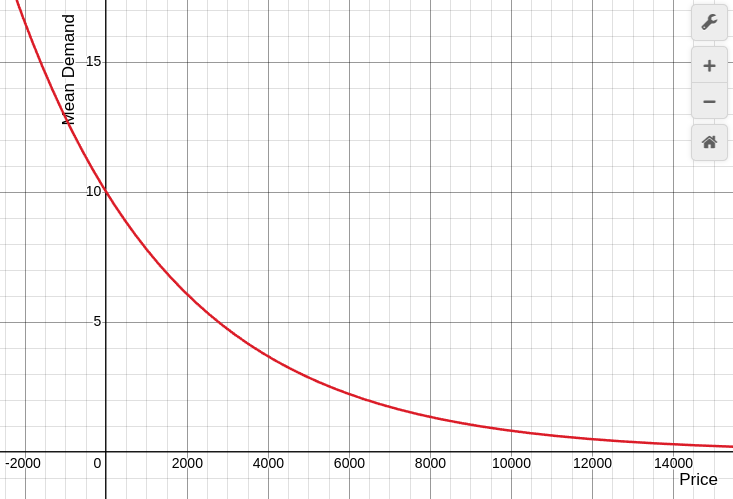
\includegraphics[width=0.5\textwidth]{mean_demand.png}
        \caption{Mean Demand at a Price \\ $\lambda(p) = 10e^{-0.00025x}$}
    \end{subfigure}
    \hfill
    \begin{subfigure}[t]{0.475\textwidth}
        \centering
        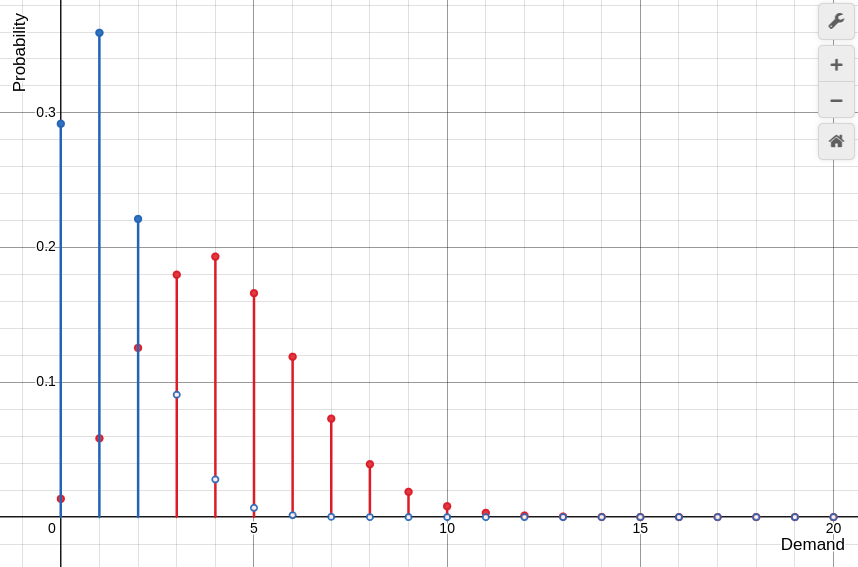
\includegraphics[width=0.5\textwidth]{demand_distribution.png}
        \caption{Demand Distribution \\ $d(p)=poisson(\lambda(p))$ \\ $p=5000 (\text{red}), 10000 (\text{blue})$}
    \end{subfigure}
    \hfill
    \caption{Demand Function}
\end{figure}
\end{frame}

\begin{frame}{Introduction: MDP Formulation}
\begin{itemize}
    \item State Space: Number of seats available for sale.
    $$\mathcal{S} = \{0, 1, \ldots K\}$$
    \item Action Space: Price of a seat on current day.
    $$\mathcal{A} = \{p_{min}, p_{min} + \Delta, \ldots, p_{min} + n \cdot \Delta\}$$
    \item Transition: Number of seats left after sale on current day.
    $$s'(s, p) = s - min(s, d(p))$$
    \item Reward: Price of all seats sold on the current day.
    $$r(s, p, s') = p \cdot (s - s')$$
\end{itemize}
\end{frame}

\begin{frame}{Introduction: MDP Formulation}
\begin{itemize}
    \item Time Horizon: Booking window of $T$ days for price adjustment and sales.
    $$\mathcal{T} = \{0, 1, \ldots T\}$$
    \item Absorbing/Terminal States: No sales can be made after the end of booking window or seats in inventory.
    $$V_0(s) = 0, \forall s \in \mathcal{S}$$
    $$V_t(0) = 0, \forall t \in \mathcal{T}$$
    where $V_t(s)$ represents the value function when we have $s$ seats in inventory and have $t$ days left in the booking window.
\end{itemize}
\end{frame}
